\documentclass[draftcls,onecolumn]{IEEEtran}

%% INCLUDING THE PREAMBLE
%%%%%%%%%%%%%%%%%%%%%%%%%%%%%%%%%%%%%%%%%%%%%%%%%%%%%%%%%%%%%%%%%%%%%%%%%%%
%                                                                         %
%                                 PREAMBLE                                %
%                                                                         %
%%%%%%%%%%%%%%%%%%%%%%%%%%%%%%%%%%%%%%%%%%%%%%%%%%%%%%%%%%%%%%%%%%%%%%%%%%%

%% PACKAGES
\usepackage[]{lineno}
%\linenumbers
\usepackage[usenames,dvipsnames]{xcolor}
\usepackage{microtype}
\usepackage[obeyDraft]{todonotes}
\usepackage{fancyvrb}
\VerbatimFootnotes
\usepackage{algorithmic}

%% GRAPHICS RELATED
\usepackage{graphicx}
\usepackage[outdir=./tmp/]{epstopdf}
\graphicspath{{../images/}{./}{./tmp/}}
\DeclareGraphicsExtensions{.eps, .pdf, .jpeg, .png,}

%% CPATION SETUP
\usepackage{float}
\usepackage{caption}
\usepackage{subcaption}
\captionsetup{belowskip=12pt,aboveskip=4pt}


%% BIBLIOGRAPHY
\bibliographystyle{ieeetr}

%% UNITS
\usepackage{siunitx}

%% EQUATIONS
\usepackage{amsmath}
%\numberwithin{equation}{section}

%% HYPERLINKS
\usepackage[debug]{hyperref}

%%%%%%%%%%%%%%%%%%%%%%%%%%%%%%%%%%%%%%%%%%%%%%%%%%%%%%%%%%%%%%%%%%%%%%%%%%%
%                                                                         %
%                             Listing Setup                               %
%                                                                         %
%%%%%%%%%%%%%%%%%%%%%%%%%%%%%%%%%%%%%%%%%%%%%%%%%%%%%%%%%%%%%%%%%%%%%%%%%%%
\usepackage{listings}
\lstset{ %
    language=C++,
    basicstyle=\footnotesize\ttfamily,
    numbers=left,
    numberstyle=\tiny\color{gray},
    stepnumber=2,
    numbersep=5pt,
    backgroundcolor=\color{white},
    showspaces=false,
    showstringspaces=false,
    showtabs=false,
    frame=single,
    rulecolor=\color{black},
    tabsize=2,
    breaklines=true,
    breakatwhitespace=false,
    title=\lstname,
    keywordstyle=\color{blue},
    commentstyle=\color{OliveGreen},
    stringstyle=\color{orange}
}
\DeclareCaptionFont{white}{\color{white}}
\DeclareCaptionFormat{listing}{\colorbox[cmyk]{0.43, 0.35, 0.35, 0.01}{\parbox{\dimexpr\textwidth-2\fboxsep\relax}{#1#2#3}}}
\captionsetup[lstlisting]{format=listing,labelfont=white,textfont=white,singlelinecheck=false,margin=0pt,font={bf,footnotesize}}
%\lstnewenvironment{code}[1][]%
%{ \noindent\minipage{\linewidth}
%	\lstset{#1}
%}
%{\endminipage}
%% USER COMMANDS
\usepackage{isotope}
\newcommand{\iso}{\isotope}
\newcommand{\figurewidth}{\textwidth}
\newcommand{\micron}{$\mu$m}


\usepackage[iso,american]{isodate}
\usepackage{ctable}
%% SUBVERSION INFORMATION
\usepackage{svn-multi}
\svnidlong
{$LastChangedBy: matthew.urffer@gmail.com $}
{$LastChangedRevision: 726 $}
{$LastChangedDate: 2013-05-16 18:55:55 -0400 (Thu, 16 May 2013) $}
{$HeadURL: https://murphs-code-repository.googlecode.com/svn/trunk/documentation/ExperimentWriteups/PMMA_UVTAcrylic.tex $}
%%%%%%%%%%%%%%%%%%%%%%%%%%%%%%%%%%%%%%%%%%%%%%%%%%%%%%%%%%%%%%%%%%%%%%%%%%%
%                                                                         %
%                                Start of Document                        %
%                                                                         %
%%%%%%%%%%%%%%%%%%%%%%%%%%%%%%%%%%%%%%%%%%%%%%%%%%%%%%%%%%%%%%%%%%%%%%%%%%%
\begin{document}
\title{Carborane Loaded Plastic Detectors}
\author{Matthew J. Urffer}
\date{\today}
\maketitle

% Tables of Contents, Figures, Tables
\tableofcontents
\listoffigures
\listoftables
%%%%%%%%%%%%%%%%%%%%%%%%%%%%%%%%%%%%%%%%%%%%%%%%%%%%%%%%%%%%%%%%%%%%%%%%%%%
%                                                                         %
%                              Start of Content                           %
%                                                                         %
%%%%%%%%%%%%%%%%%%%%%%%%%%%%%%%%%%%%%%%%%%%%%%%%%%%%%%%%%%%%%%%%%%%%%%%%%%%
\section{Introduction}

\iso[10]{B} is an attractive replacement neutron absorber ($\iso[10]{B}\left( n,\alpha \right ) \iso[7]{Li}$, Q-value \SI{2.78}{\MeV}) for radiation portal monitors because of it's high thermal cross section (\SI{3800}{b}) and ability easily incorporate into an organic scintillator.
South Carolina State University (SCSU) has prepared several methylstyrene samples containing various amounts of carborane, ranging from 0\% to 5\%.
\autoref{tab:MSSampleComp} shows the composition of these samples.
\begin{table}[h]
\centering
\caption[Methylstyrene Detectors Physical Properties]{Physical properties of the methylstyrene detectors fabricated at SCSU.}
\label{tab:PhysicalProperties}
  \begin{tabular}{m{4cm}| m{2cm} m{2cm} m{2cm} m{2cm} }
  \toprule
     Sample Name & Percent Carborane &  Thickness (mm) & Sample Mass (g) & Mass Absorber (mg)\\
    \midrule
    MS1A & 0 & 12.6 & 2.752 & 0 \\
    MS2A & 1 & 10.4 & 2.451 & 3.68  \\
    MS3A & 2 & 10.1 & 2.464 & 7.39 \\
    MS4A & 3 & 10.2 & 2.481 & 11.2 \\
    MS5A & 4 & 10.7 & 2.483 & 14.9 \\
    MS6A & 5 & 10.7 & 2.462 & 18.5 \\
    \bottomrule
  \end{tabular}
\end{table}

\section{Measured Detector Performance}
The six methylstyrene samples were tested for their alpha, beta, gamma, and thermal neutron responses in the University of Tennessee's characterization laboratory.

\subsection{Light Yield}

The alpha spectra of the films were collected using an \iso[241]{Am} source with a (predominantly \SI{5.48}{\MeV}).
\autoref{fig:LYAlpha} shows the spectra for two extremes of the methylstyrene samples compared to a commercial boron loaded scintillator, while \autoref{fig:LYAlphaMS} provides a comparison for all of the measured SCSU methylstyrene samples. 
It is observed for all of the samples that an increasing boron content decreases the light yield.
\begin{figure}
  \centering
  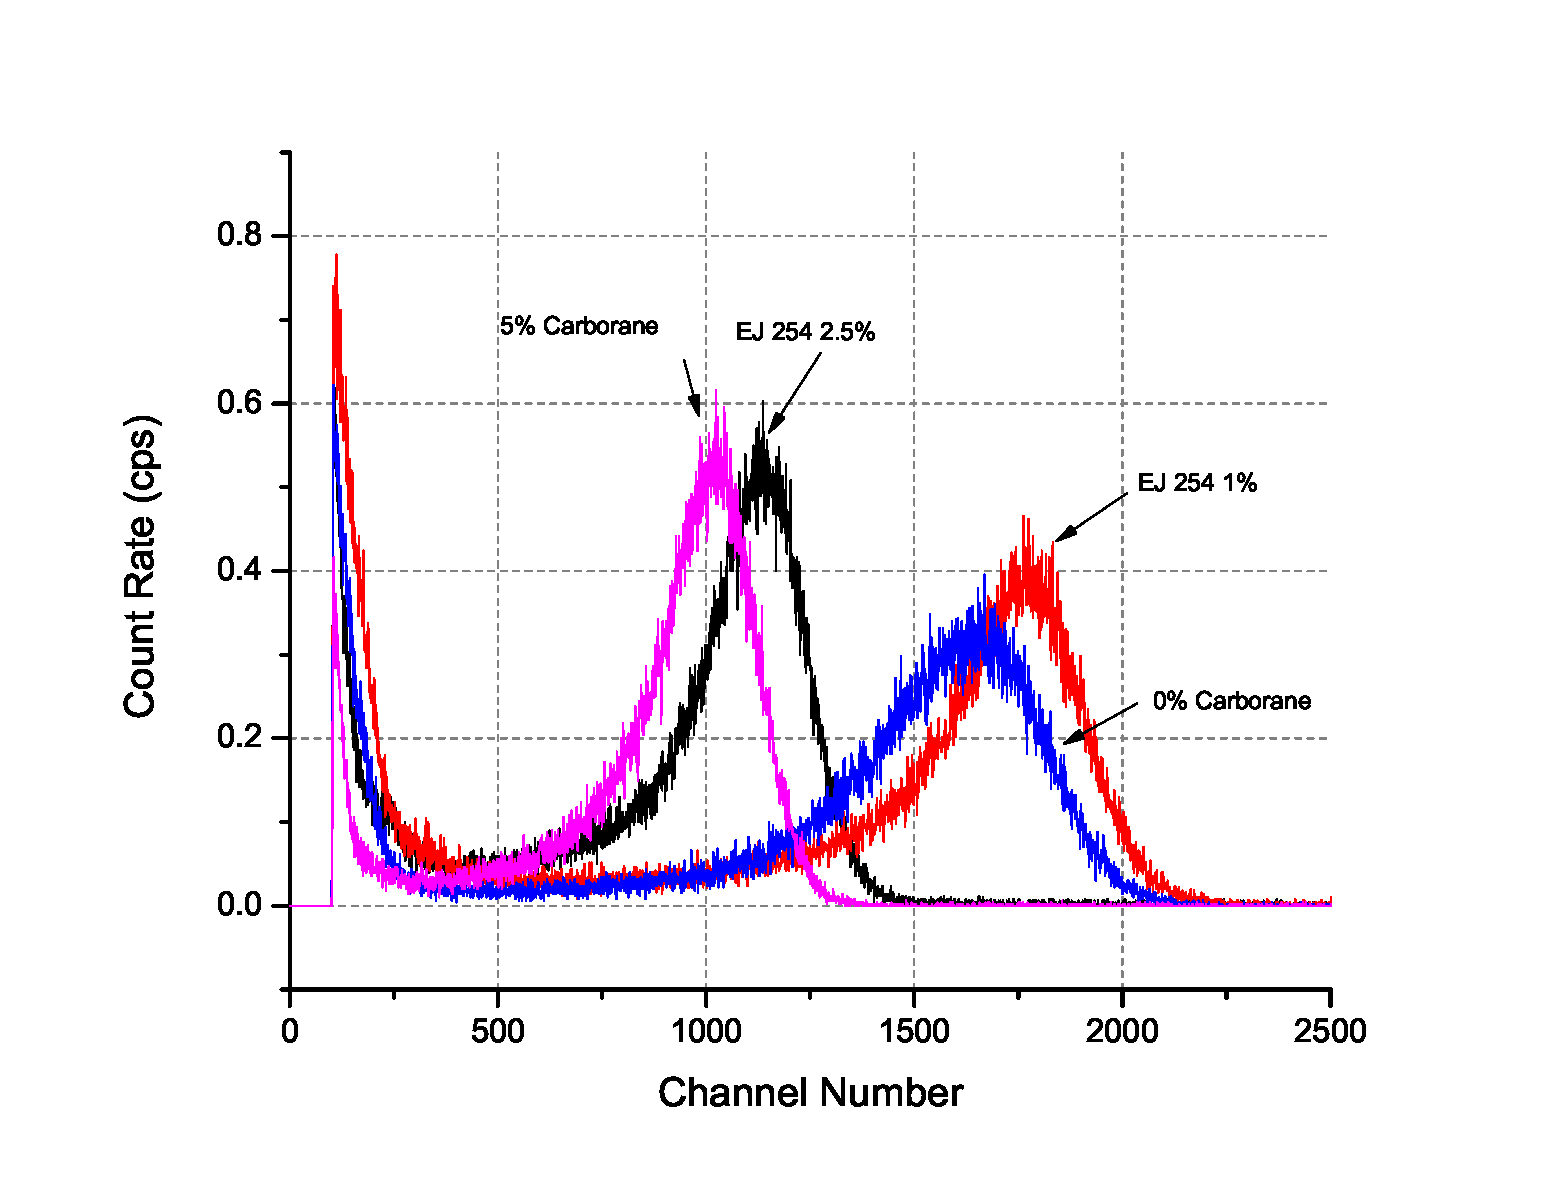
\includegraphics[width=0.6\textwidth]{MSCarborane_EJ254_Alpha-Selected}
  \caption[Alpha Response of Selected Boron Loaded Samples]{Alpha (\iso[241]{Am}) response of selected methylstyrene and commercial (EJ-254) boron loaded scintillators.  Note that in both cases the light yield is diminished as additional boron is added.}
  \label{fig:LYAlpha}
\end{figure}
\begin{figure}
  \centering
  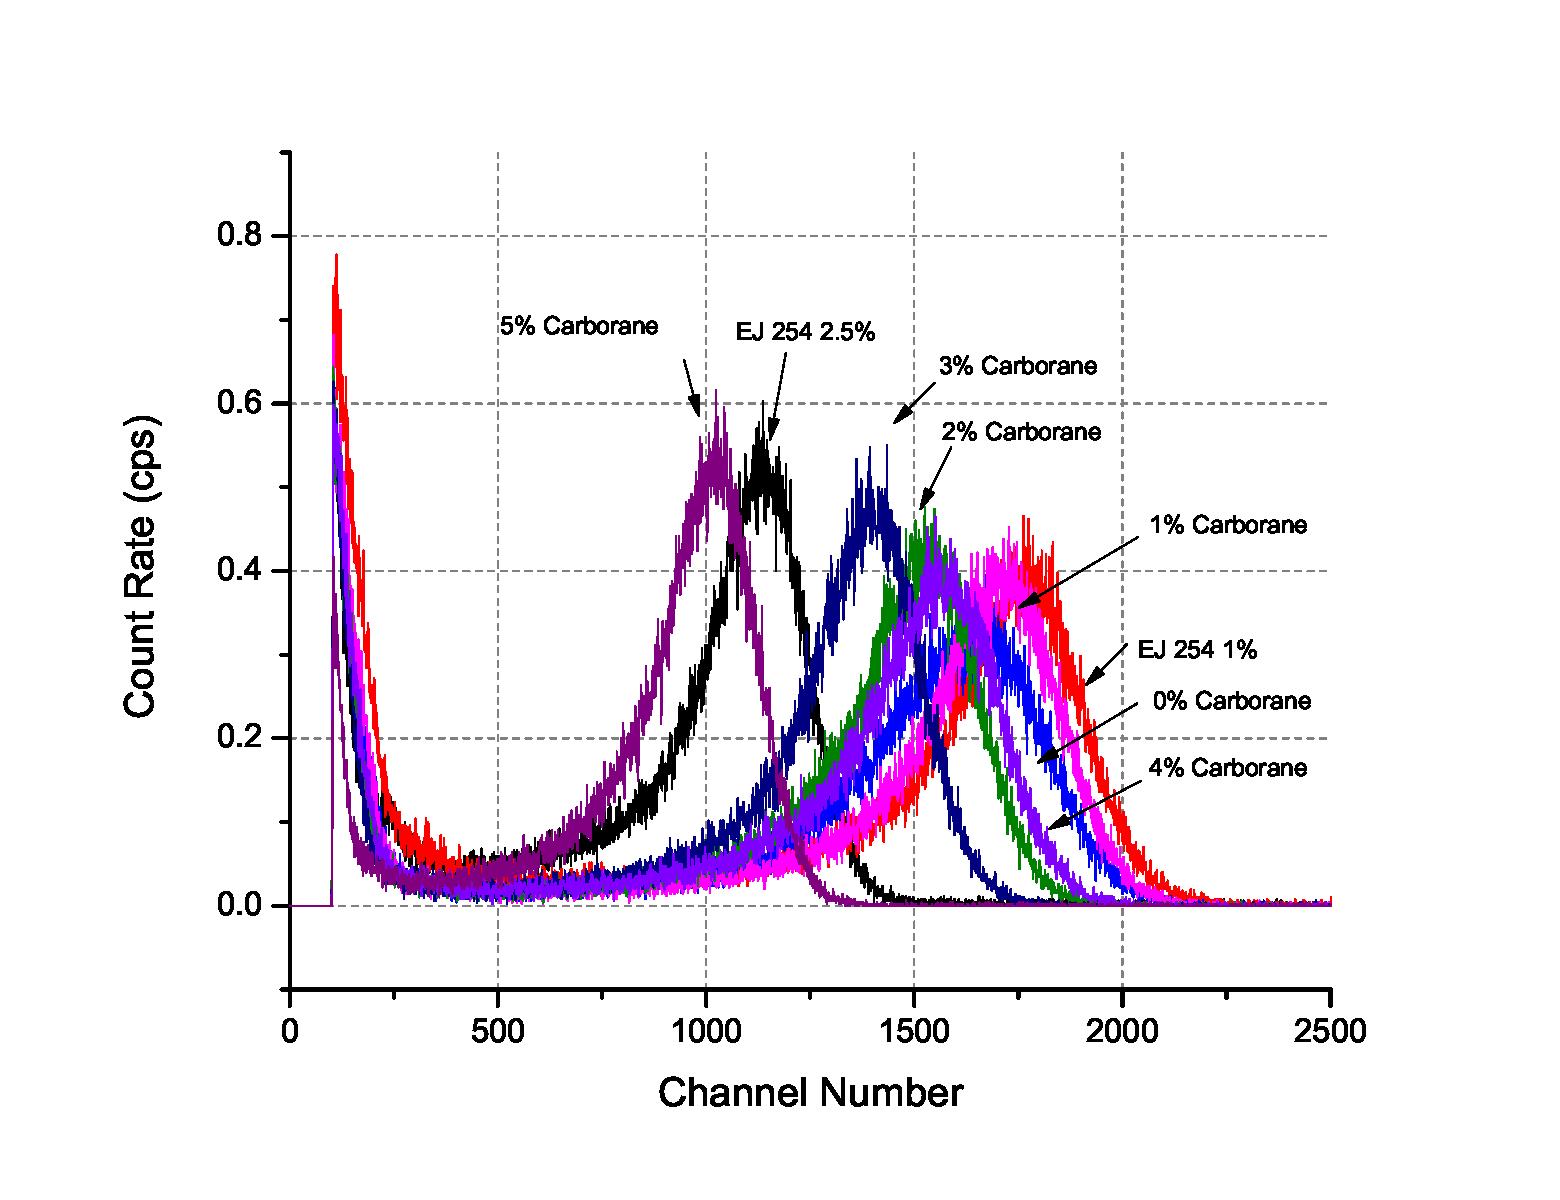
\includegraphics[width=0.6\textwidth]{MSCarborane_EJ254_Alpha}
  \caption[Alpha Response of Methylstyrene Boron Loaded Samples]{Alpha (\iso[241]{Am}) response of methylstyrene boron loaded scintillators.  Note the light yield is diminished as additional boron is added.}
  \label{fig:LYAlphaMS}
\end{figure}
\autoref{fig:LY} demonstrates the light yield from a variety of radiation sources represented by either the average of that spectra or the peak. 
The neutron average of EJ-254 1\% is 338 channels, with an alpha peak of 1,139 channels and a beta average of 765 channels.
Thus, the fabricated methylstyrene samples have a higher light output.
A rough estimate of the decrease in light yield can then be calculated from the 0\% carborane samples to the 5\% carborane samples; for alphas it is around 30\% while for \iso[60]{Co} gammas it is around 13\%, and for neutrons from 1\% to 5\% carborane there is almost 45\% decrease in the light output as calculated by the neutron average in the thermal well.
\begin{figure}
  \centering
  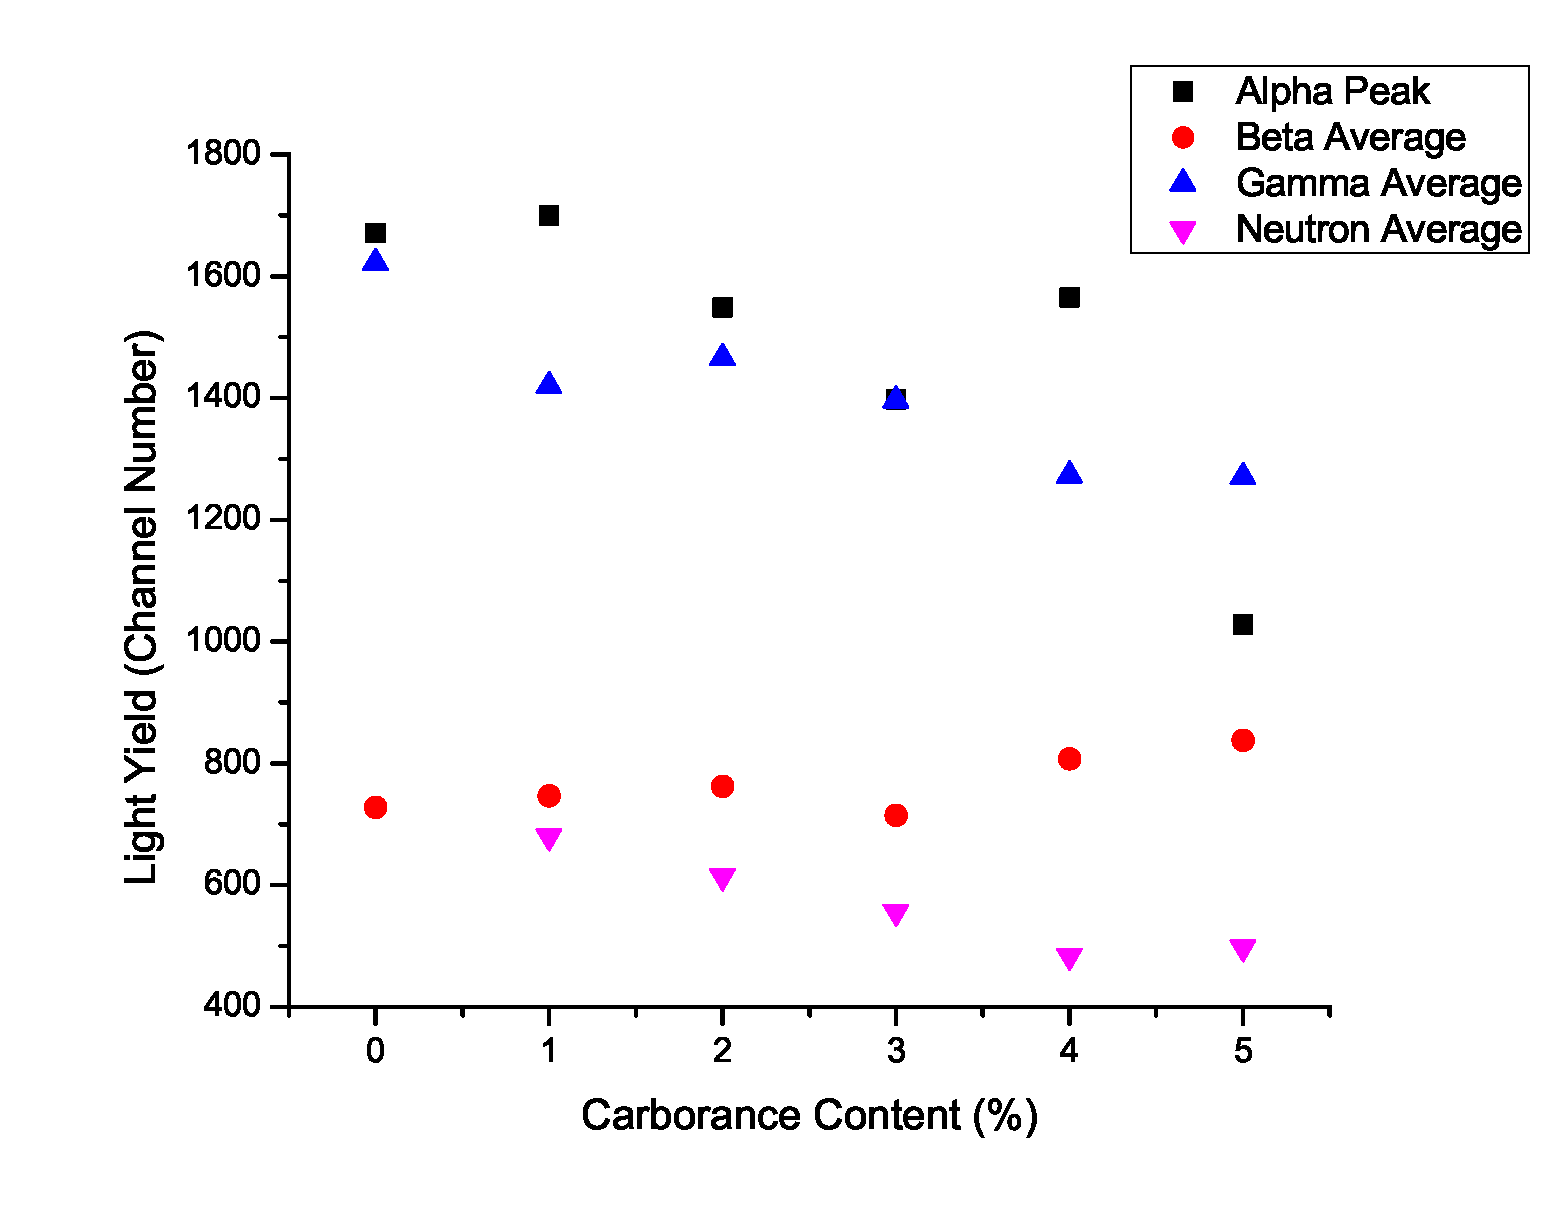
\includegraphics[width=0.6\textwidth]{MSCarborane_LightYield}
  \caption[Light Yield of Methylstyrene Carborane Samples]{Light yield (average or peak) of the methylstyrene samples for a variety of sources.  The decrease in light yield as a function of carborane content is evident. EJ-254 1\% has a published light output of \SI{9,200}{photons\per\MeV} which corresponds to a beta average of 765 channels.} 
  \label{fig:LY}
\end{figure}
\subsection{Neutron Performance}
The neutron performance of these detectors is shown in \autoref{fig:NeutronSpectra}.
The effect of adding carborane can be seen in the spectra where adding carborane tends to decrease the light yield of the sample, while increasing the total count rate.
It is also observed that these samples are brighter than the commercial EJ-254 1\% boron samples.
\autoref{fig:NCRperMass} shows the count rate of each carborane sample as a function of carborane loading, normalized by the mass of the sample. 
It is observed that very little gain in the total count is observed for four to five percent carborane loading, this is due to the self shielding and depletion of the neutron flux within the sample.
\autoref{fig:NCRper10B} shows the neutron count rate normalized by the mass of \iso[10]{B} in the sample, where the effects of self-shielding are clearly evident in the downward trend count rate per mass absorber as a function of carborane loading.
\begin{figure}
  \centering
  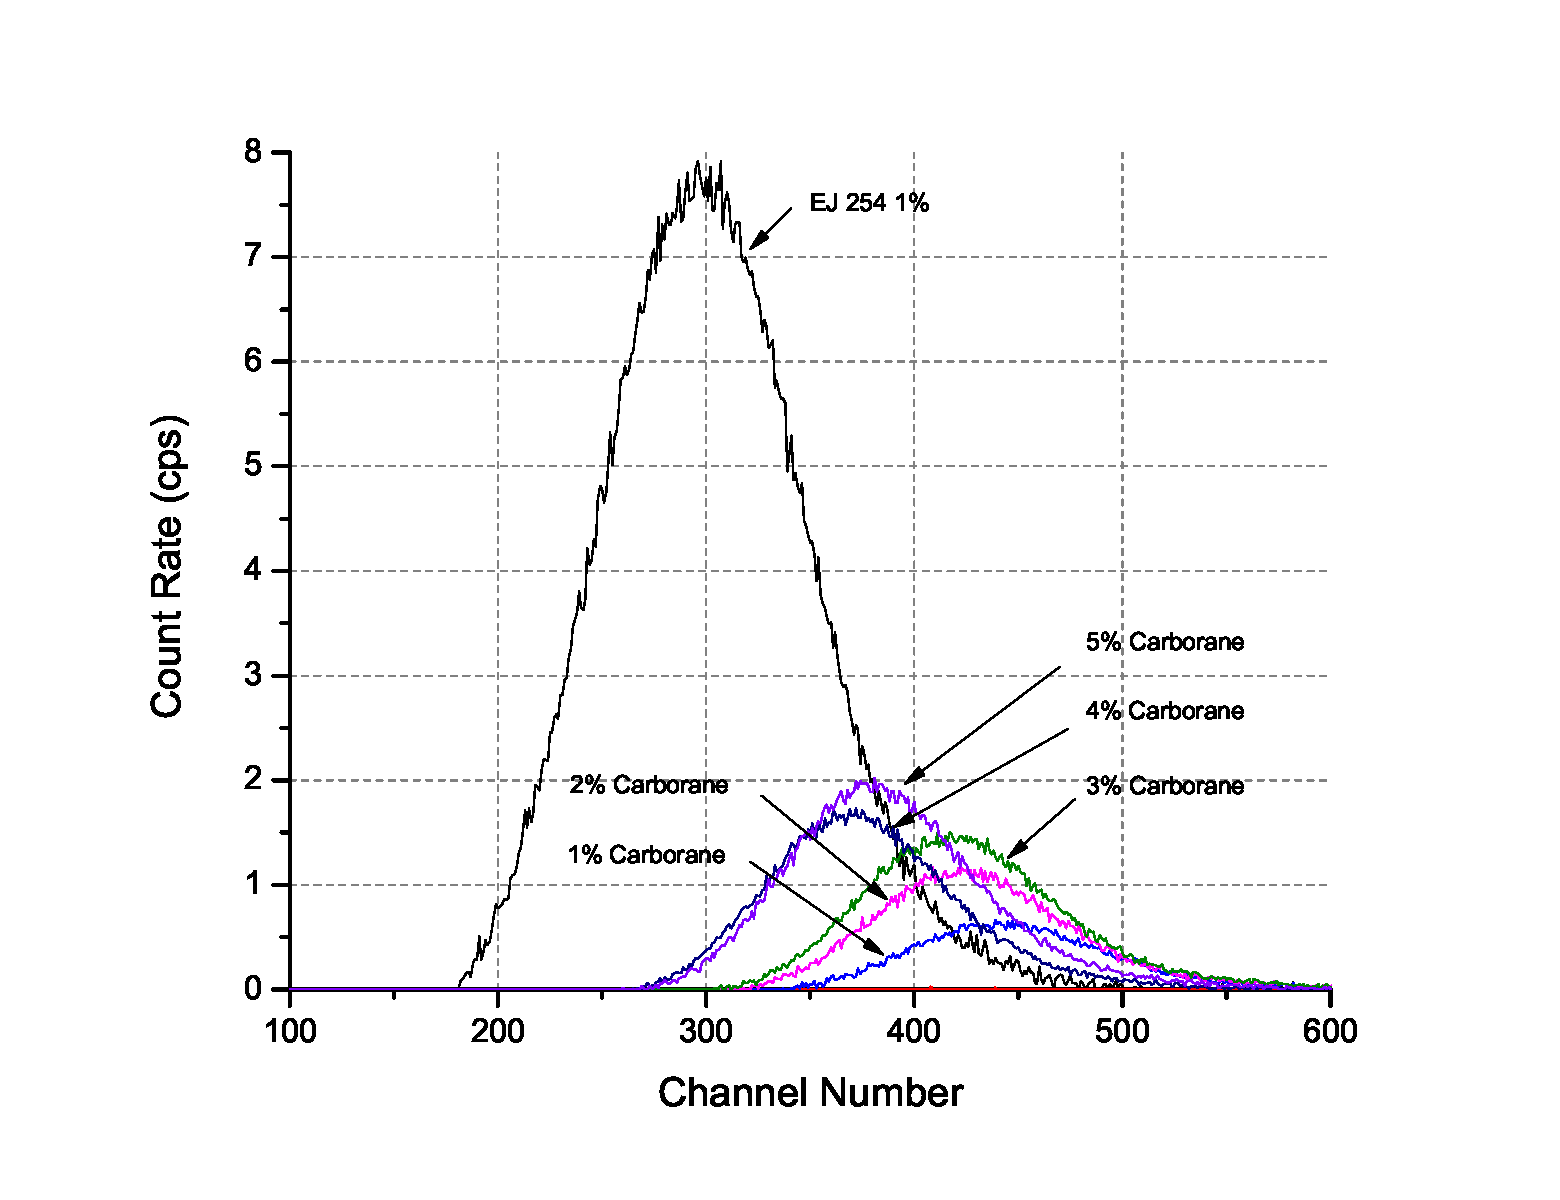
\includegraphics[width=0.6\textwidth]{MSCarborane_NetNeutron}
  \caption[Measured Thermal Neutron Count Rate]{Measured thermal neutron spectra.}
  \label{fig:NeutronSpectra}
\end{figure}
\begin{figure}
  \centering
  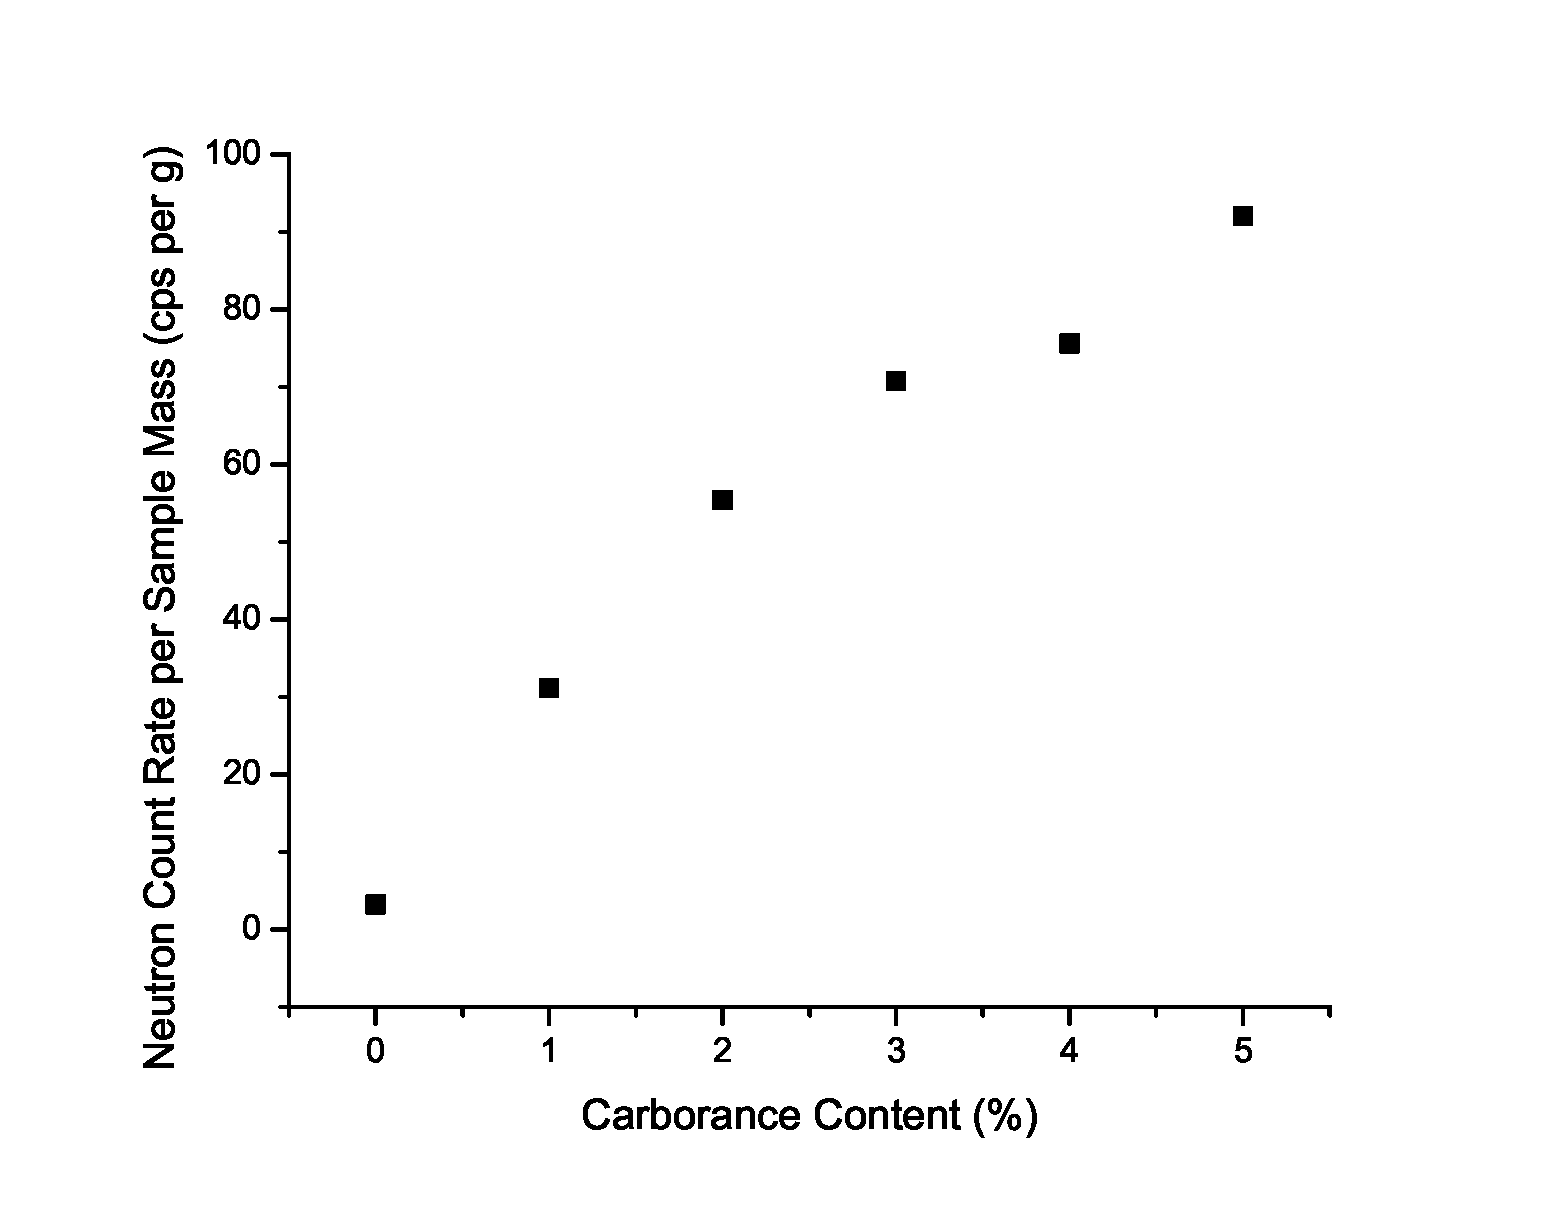
\includegraphics[width=0.6\textwidth]{MSCarborane_NetNCR_perMass}
  \caption[Measured Thermal Neutron Count Rate]{Measured thermal neutron count rate as a function of carborane concentration. }
  \label{fig:NCRperMass}
\end{figure}
\begin{figure}
  \centering
  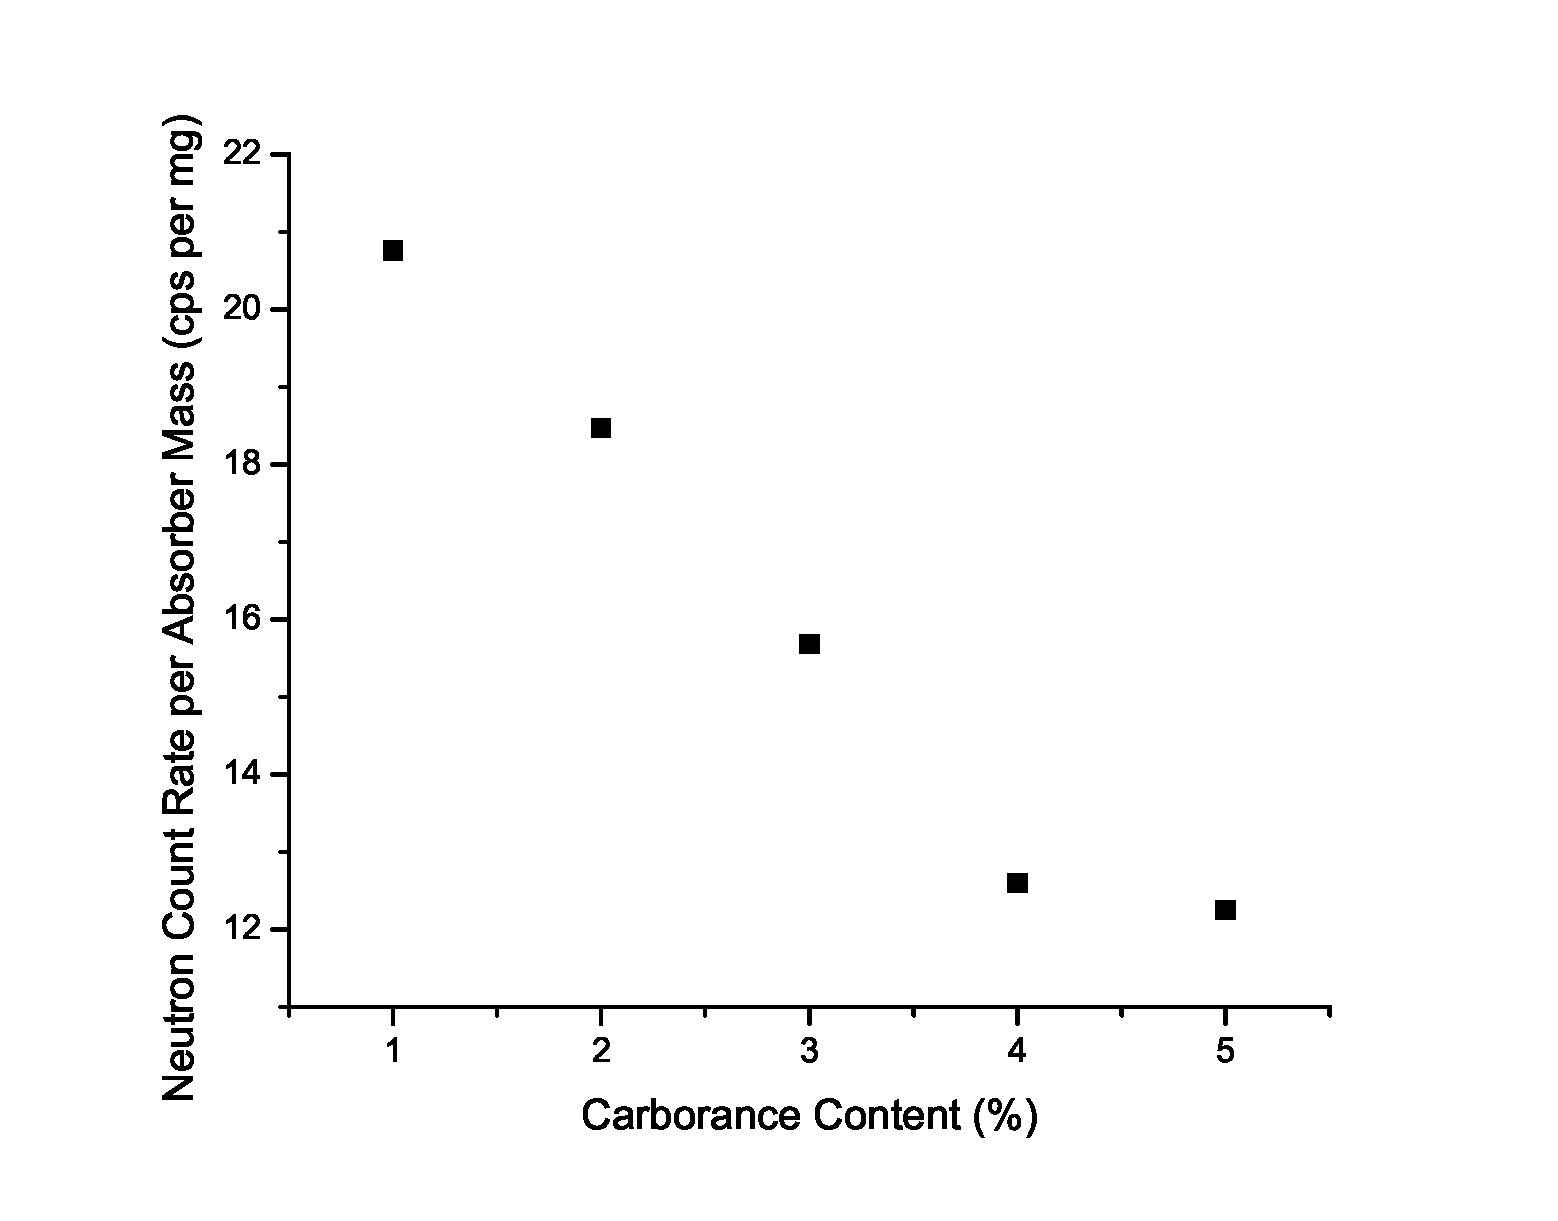
\includegraphics[width=0.6\textwidth]{MSCarborane_NetNCR_per10B}
  \caption[Measured Thermal Neutron Count Rate]{Measured thermal neutron count rate as a function of carborane concentration. }
  \label{fig:NCRper10B}
\end{figure}
\section{Proposed Experiments}
It is proposed to recast one of the samples unto disk in order to limit the energy deposition of gammas and therefore improve the neutron - photon discrimination.
\pagebreak
\appendices
\section{}
\section{File Locations and Report Status}
The spectra files for this report may be found in \path{SpectraFiles/(0)_2013_Data/PSArcylicUVT_vs_PMMA}, and the plots were generated with the OriginPro project \path{AcrylicUVT.opj}.
This document is may be found in \LaTeX format at \url{\svnkw{HeadURL}}.  
The latest revision for this file is \svnrev, and was on \svndate, committed by \svnauthor.
The films were fabricated by Andrew Mabe.
\end{document}
